%!TEX root = main_arduino_intro.tex

\chapter{Blink}

Like programming tutorials start with a ``Hello World!'' program, electronics tutorials generally start with a blink example. In this chapter you will learn how to write to and read from digital \ac{io} pins. 

\section{\Acp{led}}

\subsection{Internal \ac{led}}

Arduinos with a built-in \ac{led} allow the user to program and use this \ac{led}. Therefore, all the hardware you need is the Arduino and a USB cable in order to connect it to your computer. Feel free to plug the Arduino into a breadboard as shown in Figure~\ref{fig:blink:arduino_alone}.
\begin{figure}[htb]
    \centering
    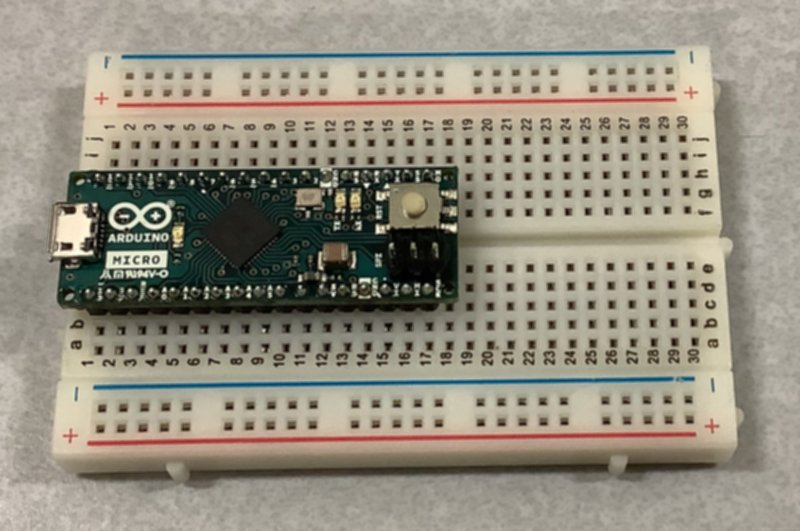
\includegraphics[width=0.6\textwidth]{graphics/01_blink/arduino_alone.jpg}
    \caption{Arduino micro plugged into a breadboard. On the left the USB connection is visible. On the right of the label where it says ``Arduino'', the internal LED can be seen.}
    \label{fig:blink:arduino_alone}
\end{figure}
The internal \ac{led} in Figure~\ref{fig:blink:arduino_alone} can be seen just on the right side of the label that says ``Arduino''. In addition, you can see a button on the right-hand side of the board (the reset button) as well as two more \acp{led} on the left side of this button. These additional \acp{led} cannot be accessed by the user and are reserved for the system.

If you start the \ac{ide} and load the basic example ``Blink'', you will get some code that will control the \ac{led}. The following exercises will use this simple example and slowly extend it.

\exerbox{Open the example blink file and read the comments. What is done in the setup? What does the variable \lstinline{LED_BUILTIN} stand for? Study the loop: What will happen when you upload the code to your Arduino? Do so and see if your assumptions were correct. Modify the timings of the program such that the \ac{led} blinks at a different rate.}

\subsection{External \acs{led}}

We can also connect an external \ac{led} to a digital \ac{io} pin. To use a pin as an output pin, i.e., to set its level by software, we have to define the \lstinline{pinMode} to be in \lstinline{OUTPUT} mode. Furthermore, connecting an \ac{led} to a pin and simply driving it can be bad for the \ac{led}, since it has, by itself, no resistance. Looking at equation~\eqref{eqn:uri} we can see that in such a case the current should become infinity, which might destroy the \ac{io} pin. Fortunately, Arduinos have an internal resistor that prevent this from happening. However, the \ac{led} might still get too much current, which might significantly reduce its lifetime. You can either add a resistor or use an LED with an internal one, as we are doing here (Figure~\ref{fig:blink:arduino_led}).

\begin{figure}[htb]
    \centering
    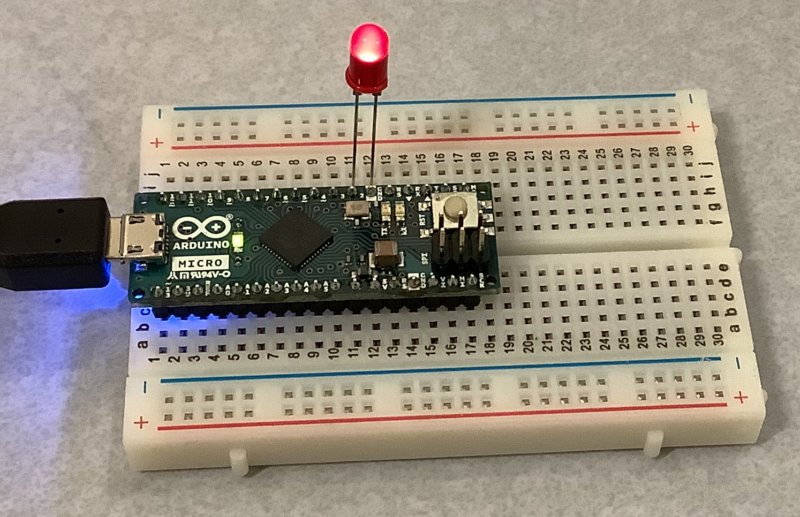
\includegraphics[width=0.6\textwidth]{graphics/01_blink/arduino_led.jpg}
    \caption{Arduino with one \ac{led} connected.}
    \label{fig:blink:arduino_led}
\end{figure}
\exerbox{Draw a wiring diagram to connect your own \ac{led} to a Arduino output pin. Where do the anode and cathode of the \ac{led} connect to? Attach your \ac{led} to the arduino and modify the simple blink experiment to use your \ac{led} instead of the built-in one. If you have trouble figuring out how to connect the \ac{led}, study Figure~\ref{fig:blink:arduino_led} and remember that every electric circiut must be completed.}

\subsection{Dimming an \ac{led}}

As we have discussed above, \acp{led} cannot be dimmed in the traditional way, i.e., by using a potentiometer to lower the voltage. However, we can use a \ac{pwm} output in order to only have the \ac{led} on for a certain amount of time. This will result in our brain perceiving the \ac{led} as dimmed. We have already described the \ac{pwm} outputs above in Section~\ref{sec:intro:dac}, see also Figure~\ref{fig:intro:pwm}. In order to identify a \ac{pwm} output, look at the pinout (Appendix~\ref{app:pinout}). Digital pins indicated with $\sim$ are the ones that can be used in this fashion, e.g., pin 3.

\exerbox{Connect your \ac{led} to a \ac{pwm} output pin. From the Arduino \ac{ide}, load the basic example named ``Fade''.
\begin{enumerate}
    \item Read the setup and loop functions. How is the pin output set and what is different from how the pin was set in the previous exercise?
    \item Modify the fade amount to 7 and run it again. At the brigthest point, the \ac{led} briefly blinks. Why?
    \item Can you rewrite the routine in order to prevent it from blinking at the highest point? An \href{https://www.arduino.cc/reference/en/language/structure/control-structure/if/}{\lstinline{if} statement} might be useful.
\end{enumerate}}

The \lstinline{void loop()} function acts as an endless loop. The most commonly used looping structures are \href{https://www.arduino.cc/reference/en/language/structure/control-structure/while/}{\lstinline{while}} and \href{https://www.arduino.cc/reference/en/language/structure/control-structure/for/}{\lstinline{for}} loops. In fact, the loop function iself underneath is a \lstinline{while(true)} loop.

\exerbox{Inside the \lstinline{void loop()} function, write a \lstinline{for} loop to replace the ramp. Ensure that your loop does not blink, even if you select various fade amounts.}

\qbox{
    \begin{itemize}
        \item How does integer division in \cpp\ work?
        \item How can you do a division in \cpp\ and round the result to the nearest integer?
        \item What is a boolean variable and how do you compare two booleans, e.g., in an \lstinline{if} statement?
        \item How would you flip the state of a boolean variable?
    \end{itemize}
}

\subsection{Multiple \acp{led}}

\begin{figure}[tb]
    \centering
    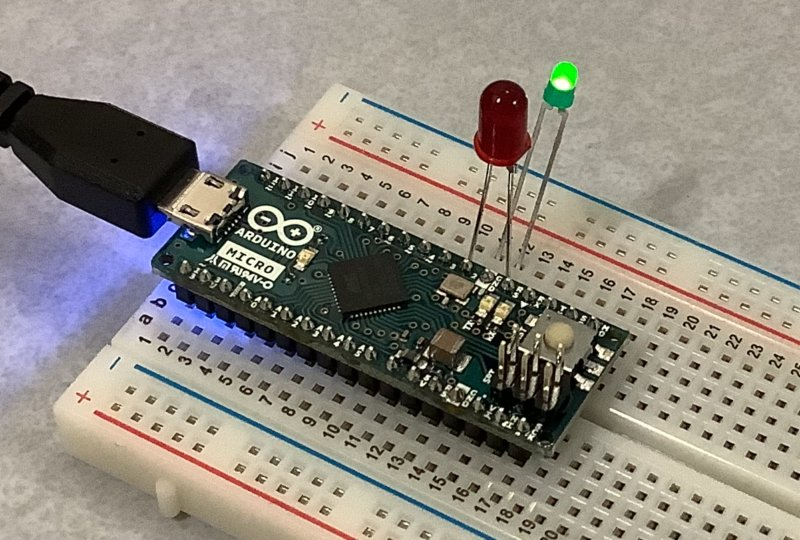
\includegraphics[width=0.5\textwidth]{graphics/01_blink/arduino_two_leds.jpg}
    \caption{An Arduino with two \acp{led} connected.}
    \label{fig:blink:arduino_two_leds}
\end{figure}
Since you have more than one pin available, multiple \acp{led} can be set up. An example of a test setup is shown in Figure~\ref{fig:blink:arduino_two_leds} This can be especially useful if you want to display the status of your setup using different colored \acp{led}.

\paragraph{Subfunctions in \cpp} Sometimes it is useful to put some of your code into external functions, i.e., not to write them into the main loop. For example, you can write a function as following:

\begin{lstlisting}
void myFunction(bool toggle) {
    // your code here...
}
\end{lstlisting}
You can then call this function from the main loop by calling \lstinline{myFunction(true);} if you want to assign the value \lstinline{true} to the variable \lstinline{toggle}.

\exerbox{Setup two \acp{led}, a red and a green one. Write a program that switches between blinking the red and green \acp{led}. Write a subroutine that takes a boolean variable as an input and, depending on the value of this input variable, turns either the red or the green \ac{led} on (and the other one off).}

\section{Buttons}

\begin{figure}[tb]
    \centering
    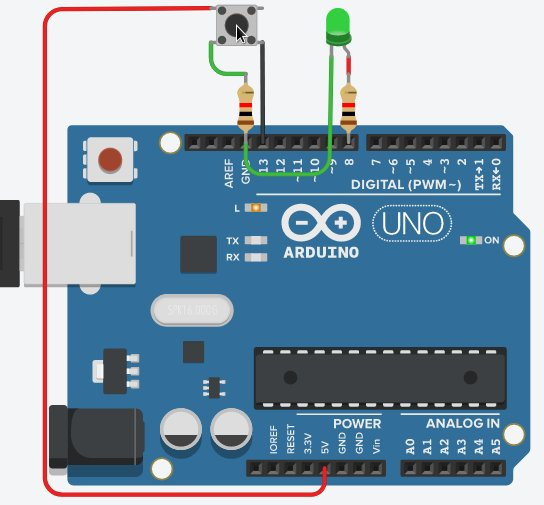
\includegraphics[width=0.45\textwidth]{graphics/01_blink/arduino_button_led_tinkercad.jpg}
    \caption{\href{https://www.tinkercad.com/things/5VP2mIHUOxB}{TinkerCAD simulation} of Arduino with a button and \ac{led} connected.}
    \label{fig:intro:button_led}
\end{figure}
Most devices that allow for user interactions contain some buttons. We can use the digital \ac{io} pins in order to connect a button. Figure~\ref{fig:intro:button_led} shows a \href{https://www.tinkercad.com}{TinkerCAD} simulation of an Arduino with a button and an \ac{led} connected. Here, we connect the button on one side to the 5\,V output of the Arduino and the other side via a 1\,k$\Omega$ resistor to ground and simultaneously to a digital \ac{io} pin. The resistor limits the current to 5\,mA, see equation~\eqref{eqn:uri}. In the setup routine, we need to set the \lstinline{pinMode} to \lstinline{INPUT}, since we want to read the value that is connected to the pin. If the button is unpressed, the pin is on the same electrical potential as ground and therefore in a low state. If the button is pressed however, the pin is at 5\,V and thus in a high state. In the loop you can, e.g., read the state of the button connected to \lstinline{buttonPin} as:
\begin{lstlisting}
int buttonState = digitalRead(buttonPin);
if (buttonState == HIGH) {
    // the button is pressed
} else {
    // the button is not pressed
}
\end{lstlisting}

\exerbox{Connect a button and an \ac{led} to your Arduino and write a program that turns the \ac{led} on while the button is pressed. Then adjust your routine such that, whenever you press the button, the \ac{led} is turned on for 3\,s and then turns off after the time has elapsed.}

\morebox{Adding time}{In the second part of the above exercise, you have (most likely) written your program such that if the button is pressed while the \ac{led} is on, nothing happens. The light will still turn off once the set time elapses after the initial button press. Can you come up with code that would allow you to reset the countdown when pressing the button again, i.e., add time to the timer?}